\chapter{Applications and Case Studies}

As the previous chapters have shed light on the process of algorithmic and thermal design; mainly in theory, illustrating the basic concepts; this chapter will delve into the practical tools used in the process, which will facilitate input of algorithms into the modelling process. Afterwards, a showcase of previous experiments with algorithmic design by either performative or generative tools

\section{Algorithm and Value Entry}

\subsection{End-user Programming}

The term ``End-user'' is used to refer to the final user of the computer application. The programming input method for the end-user is called \emph{scripting}, which allows end-user to participate in the development of the programme to add unique functionality; therefore, transferring some of tasks traditionally assigned to the software developer to the end-user.

Although scripting allows end-users to introduce new functionality, it does not mean that users would be creating new software. Scripting allows end-users to access the underlying structure of existing software and embed new functionality in it. This type of input allows for extended expressive control and higher productivity in the design process. \cite{kashyap01}

Scripting is very similar to traditional programming procedure; entering a series of instructions written in computer code, and executed within the software environment. Some popular scripting languages and their corresponding model oriented software environments include: 

\begin{enumerate}
\item AutoLisp for AutoCAD
\item RhinoScript for Rhinoceros
\item MEL for Maya
\item MAXSCRIPT for 3DsMax
\end{enumerate}

\subsection{Parametric Modelling}

Parametric Modelling is a system where a 3D geometric model has parametric attributes subject to variation, modification is usually done through numerical input of the variable value (refer to section \ref{sec:GeoModel} on parametric modelling). The model is also built with constraints that ensure that some aspects of the model are not altered, or that some are automatically changed when others are in the process of parameter or variable value change. Parametric modelling offers flexibility of change to the design; the model in this case could be called a \emph{smart} CAD model \cite{kashyap01}.

Another form of parametric modelling is generative parametric graphical modules, which analyse and decompose geometry into elements which can be controlled as input and output data into processes which ultimately affect the model. A prominent example is Grasshopper plugin for Rhinoceros.

Parametric models are of great value to performative oriented design processes, which is sometimes fused with scripting, benefiting from both in speeding the process and achieving better results.

\clearpage
\section{Case Studies}

\subsection{Adaptable Responsive Architecture}

The following will showcase a number of experiments by Alejandro Zulas \cite{zulas04}, utilising scripting to create adaptable responsive enclosure systems with emphasis on sunlight incidence.

\subsubsection{The Mutable Curtain}

The author attempted the design of a box capable of modulating light going through it (fig. \ref{fig:AZulasEncl}), which was done using Rhinoceros modelling program and its scripting language; \emph{Rhinoscript}. The experiment was an attempt to create an adaptive, responsive enclosure system which responded to solar incidence angles. 

\begin{figure}[htbp]
\centering
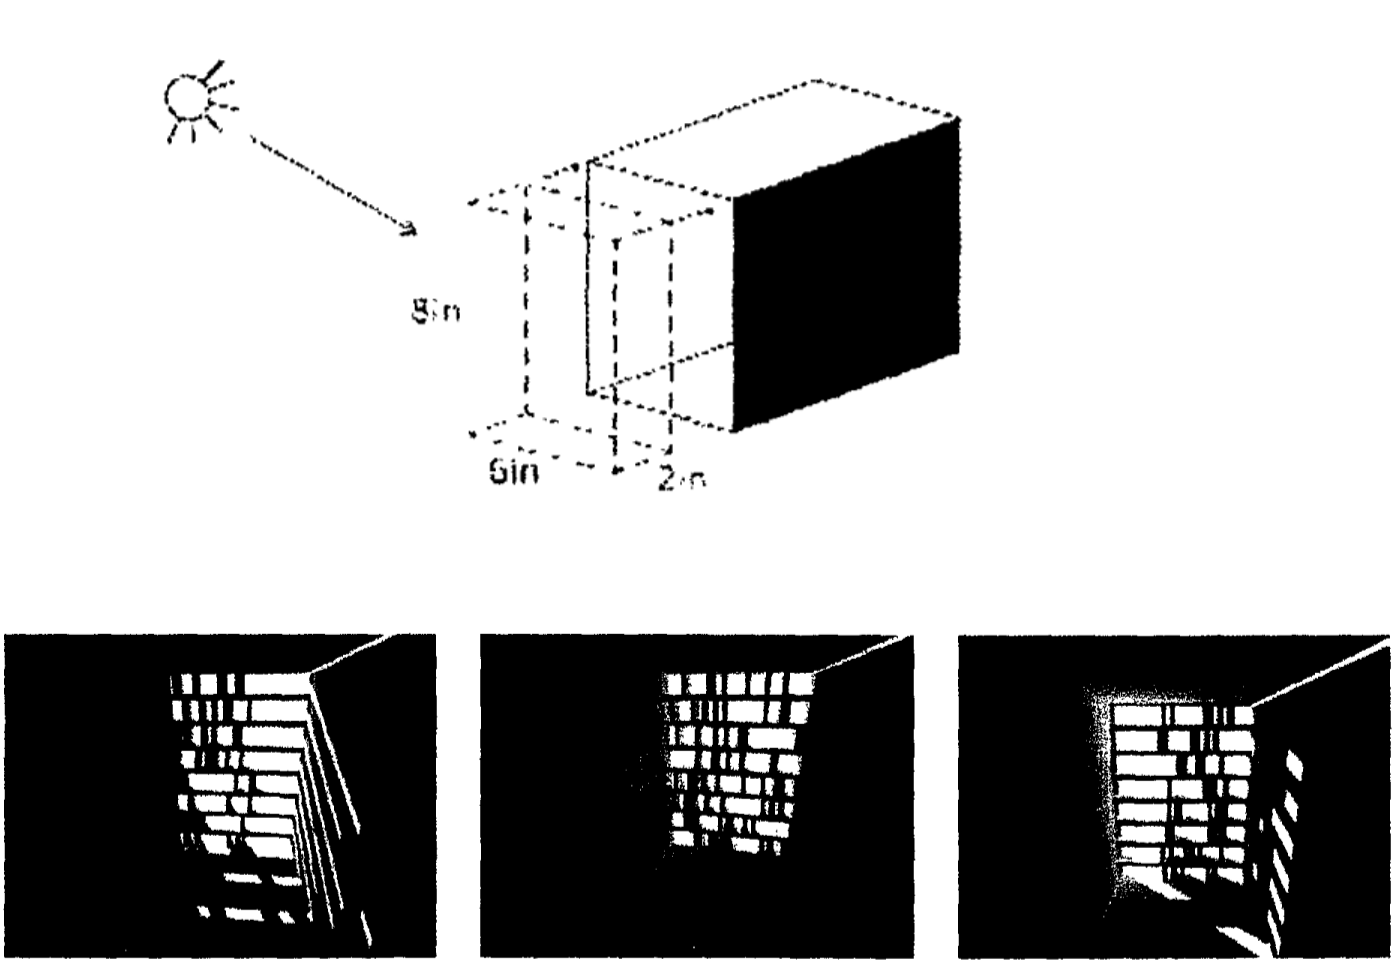
\includegraphics[width=\textwidth]{./Images/1-Enclosure}
\caption[Responsive Adaptable Enclosure Experiment]{The Enclosure and Results \cite{zulas04}}
\label{fig:AZulasEncl}
\end{figure}

The main variable in the experiment was the ratio of enclosure wall solid and void. Using an advanced draughting engine such Rhino and scripting language such as Rhinoscript, the researcher was able to create a responsive system with a generative random function to regulate the amount of light penetrating the enclosure (fig. \ref{fig:TransSeq}).


\begin{figure}[htbp]
\centering
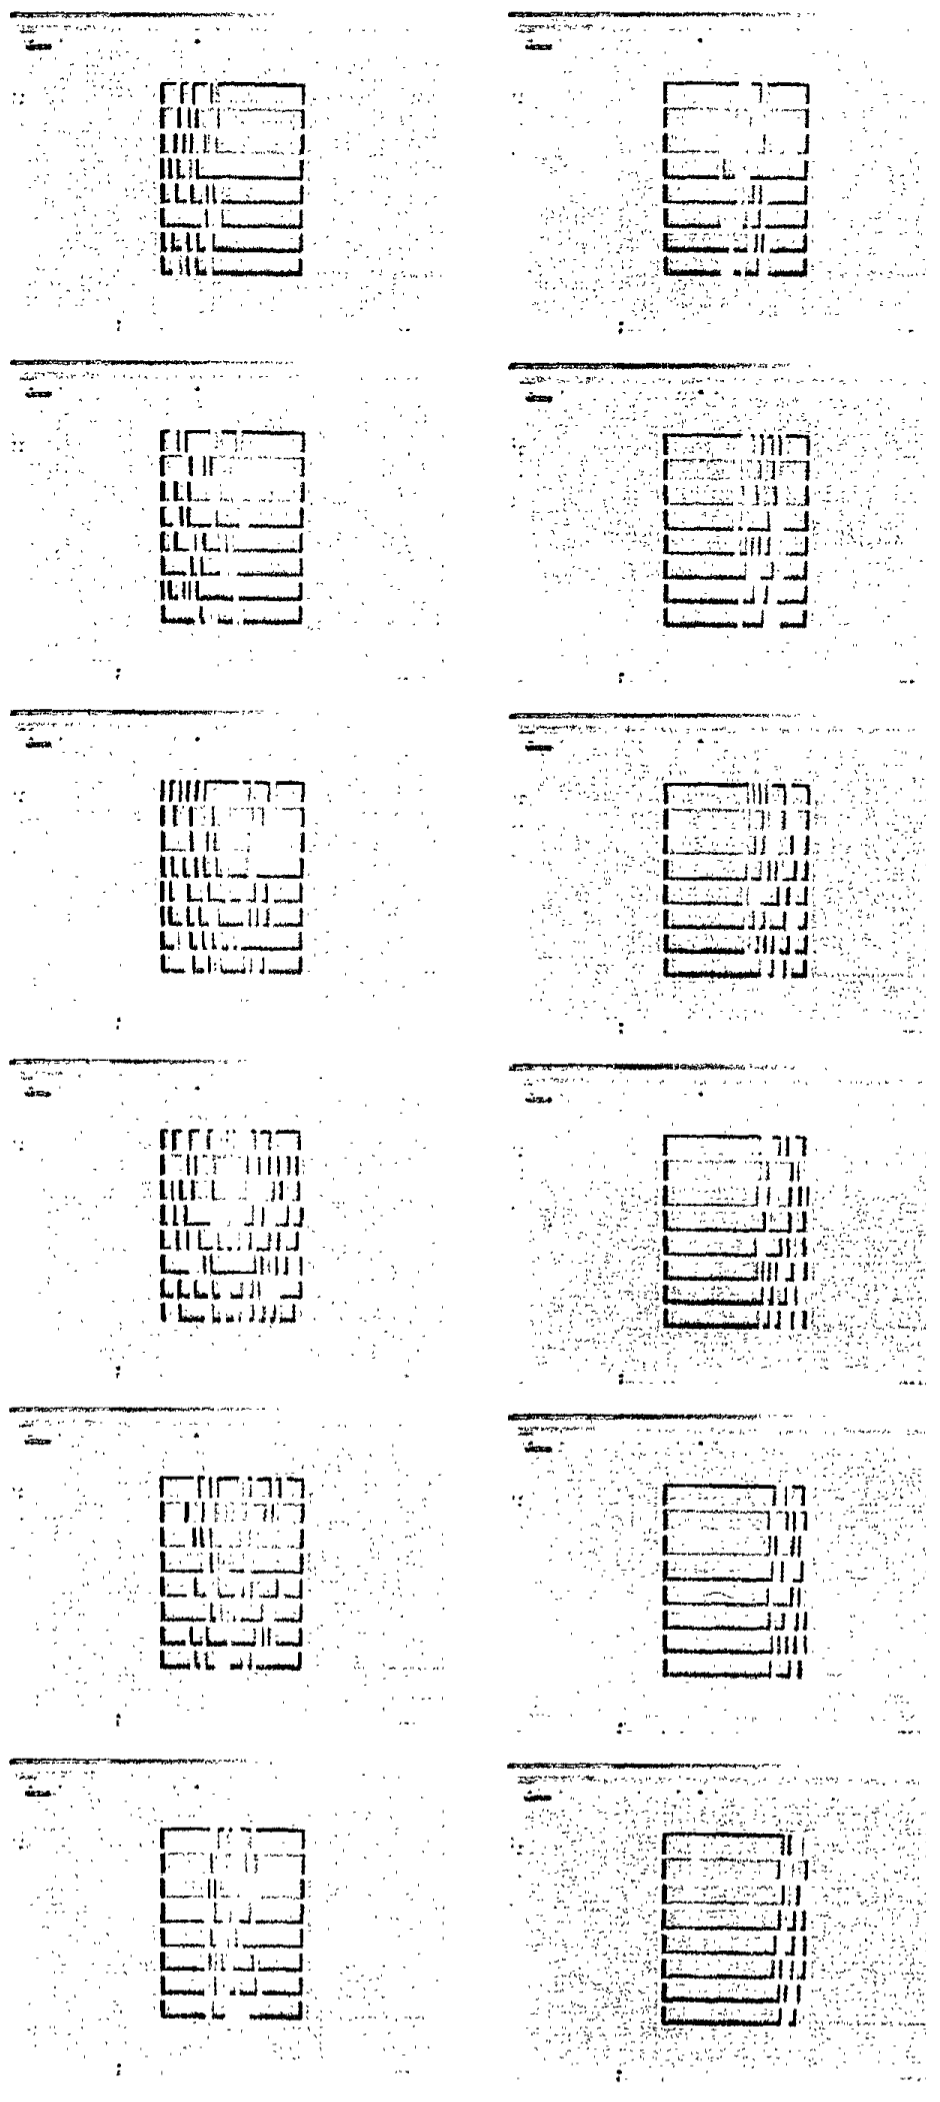
\includegraphics[height=17cm]{./Images/2-TransfSequ}
\caption[Transformation Sequence of Enclosure]{Transformation Sequence \cite{zulas04}}
\label{fig:TransSeq}
\end{figure}

\subsubsection{Responsive Louvres System}

Another experiment by the same author \cite{zulas04} was done using a parametric design driven program called CATIA (Computer Aided Three-Dimensional Interactive Application). The objective of this exercise was also to modulate light at the enclosure level, but through shading. The researcher used a number of vertical and horizontal louvres which responded to two factors; the location of the sun throughout days of different seasons which would affect the arrangement of the louvres, in addition to the angle of incidence which affected the orientation of each louvre as to reflect the light in a direction away from the building. 

The parametric CAD program, CATIA; had some advantages over Rhinoscript as it displayed the effect of any amendments to the script interactively in the form of graphical feedback, which was beneficial to the process. 

\subsubsection{Adaptable Pavilion}
\label{sec:AdptPav}

Another experiment using CATIA; an attempt to design a temporary exhibition pavilion \cite{zulas04}. The exercise focuses on the conception of a contextual responsive building addressing different variations on the overall building form and envelope in relation to sunlight. 

\begin{figure}[htbp]
\centering
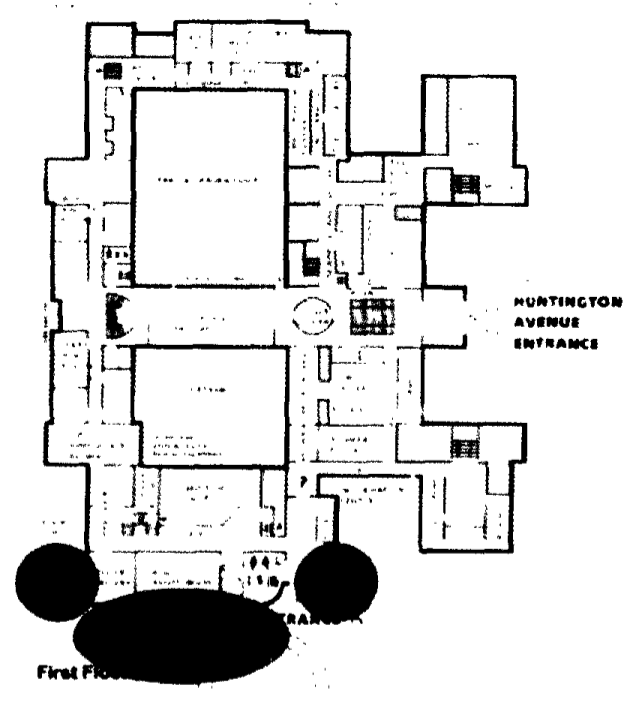
\includegraphics[width=0.5\textwidth]{./Images/4-Location}
\caption[Case Study Location]{Pavilion Location \cite{zulas04}}
\label{fig:PvlLoc}
\end{figure}

\paragraph{Design Intentions:} 

\begin{enumerate}
\item Generate an appropriate enclosed environment for the sculptures to be exhibited.
\item Implementation of a responsive louvre system as a filter to redirect light incidence inside the pavilion.
\item Analysing the behaviour of the building towards conceiving a sun responsive building (fig. \ref{fig:DesignInt}). 
\end{enumerate}

\begin{figure}[htbp]
\centering
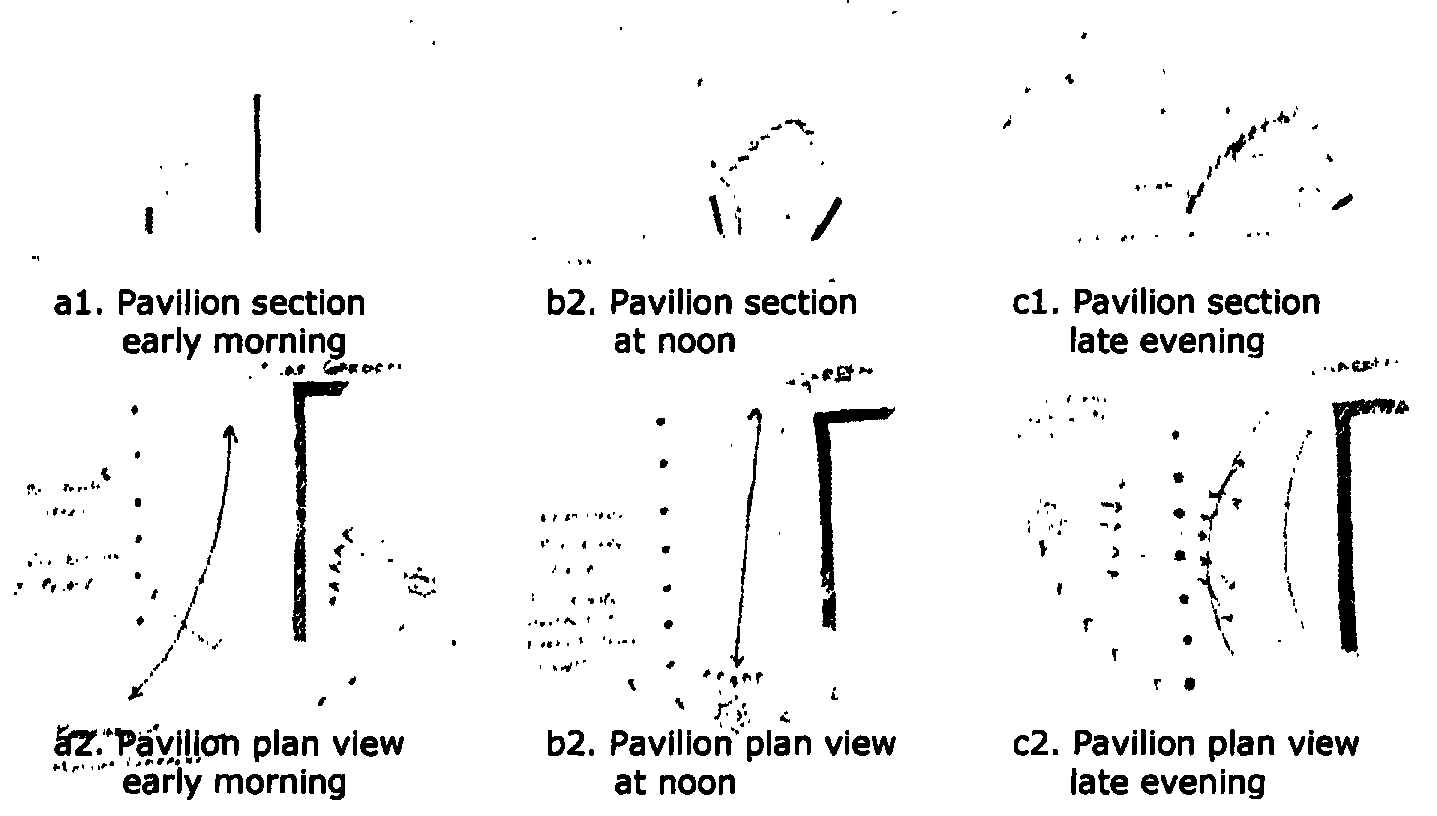
\includegraphics[width=\textwidth]{./Images/3-DesignIntent}
\caption[Pavilion Design Intentions]{Design Intentions \cite{zulas04}}
\label{fig:DesignInt}
\end{figure}

The context consisted of the sun, the museum wall and trees defining the yard. The museum wall and the trees were defined as static elements of the context, while the sun was understood as a dynamic element; this was to be taken into consideration as input. The main variables taken into consideration were the pavilions shape, length, height, proportions\ldots etc. 

Object relations were programmed using conditional ``\emph{if : then \dots else : that}''. In other words; \emph{if} the location of the sun in relation to its day-path is ``\emph{n}'', \emph{then} the line defining the pavilion's profile gets increased or decreased or rotated or thickened\ldots etc, by a predefined ``\emph{n}'' factor. (Refer to fig. \ref{fig:MpRlt})

\begin{figure}[htbp]
\centering
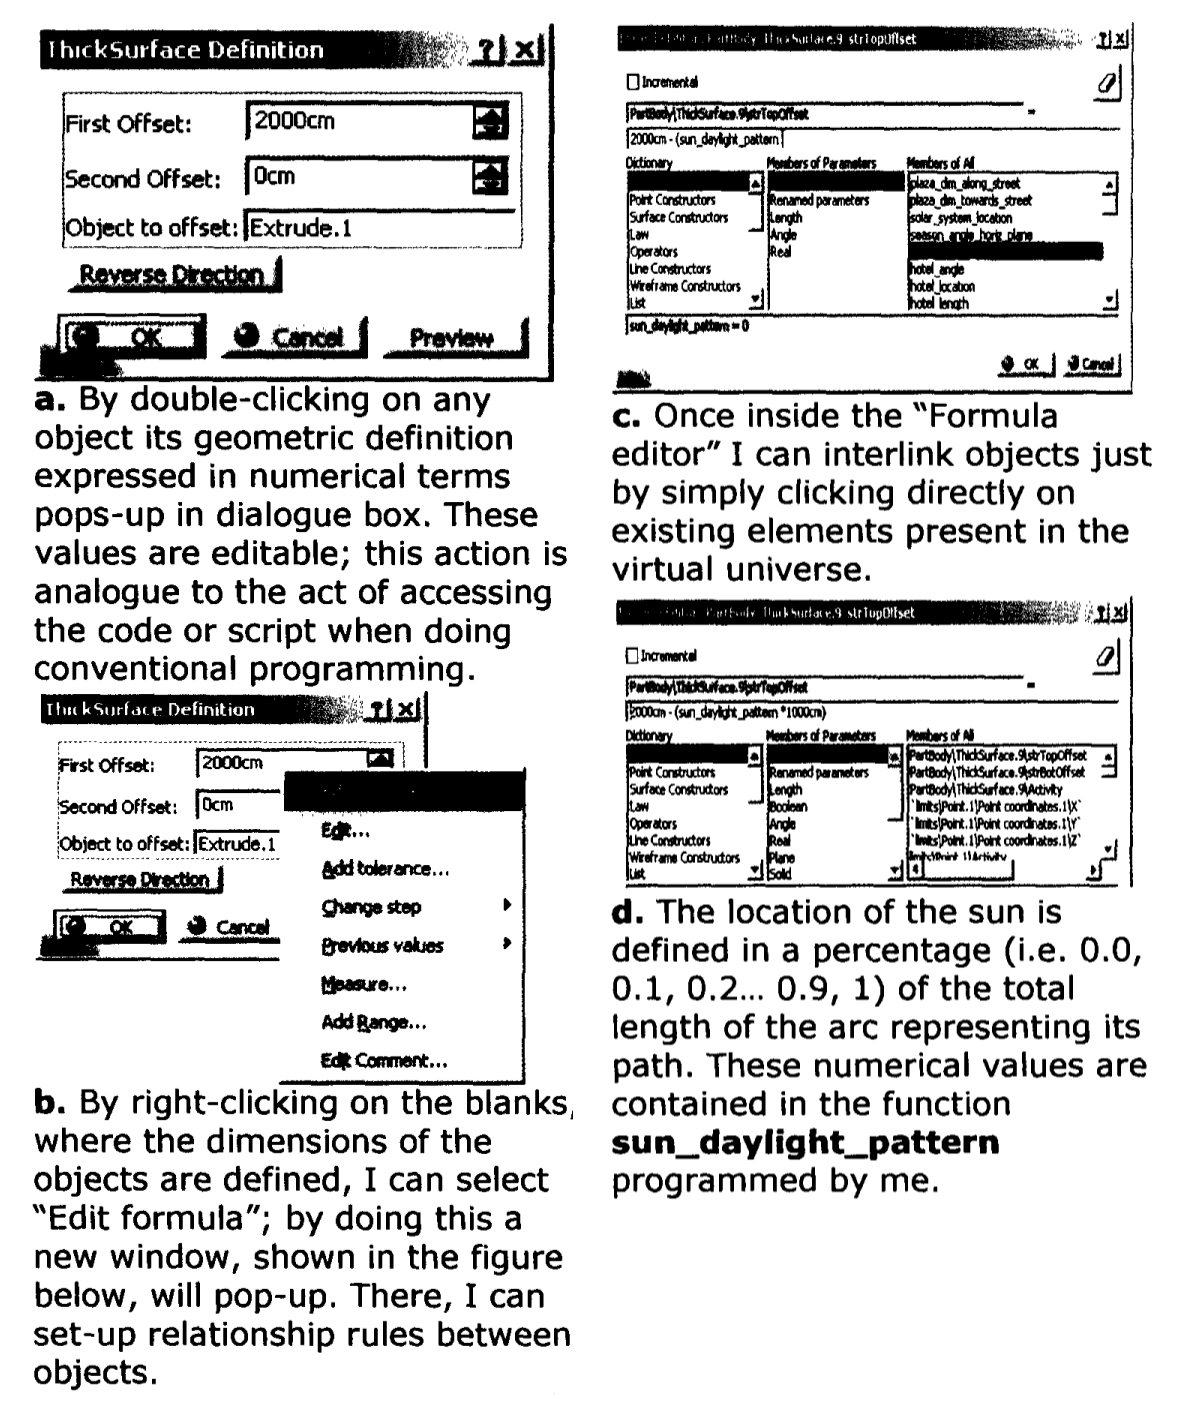
\includegraphics[width=\textwidth]{./Images/5-MappingRelations}
\caption[Mapping Design Relations]{Mapping Relationships \cite{zulas04}}
\label{fig:MpRlt}
\end{figure}

The interactiveness of CATIA was quite notable when the author attempted to change the location of the sun by means of a graphical slider and witnessed real-time changes to building shape due to the change in solar location (fig. \ref{fig:IntActCAT})

\begin{figure}[htbp]
\centering
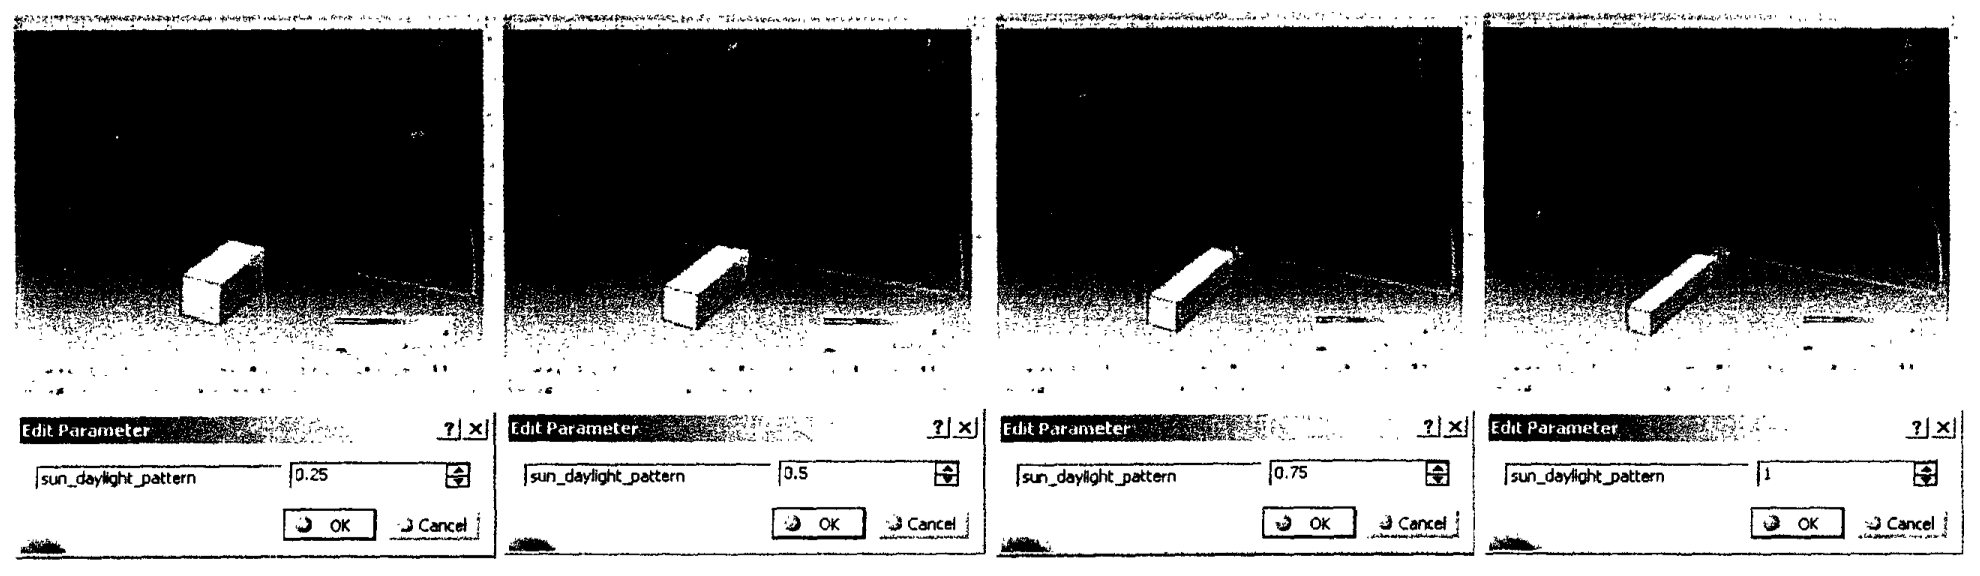
\includegraphics[width=\textwidth]{./Images/6-InteractiveCATIA}
\caption[Interactive Response]{Automated Adaption \cite{zulas04}}
\label{fig:IntActCAT}
\end{figure}

The end result was quite similar to the initial design intentions (fig. \ref{fig:FinalPav}).

\begin{figure}[htbp]
\centering
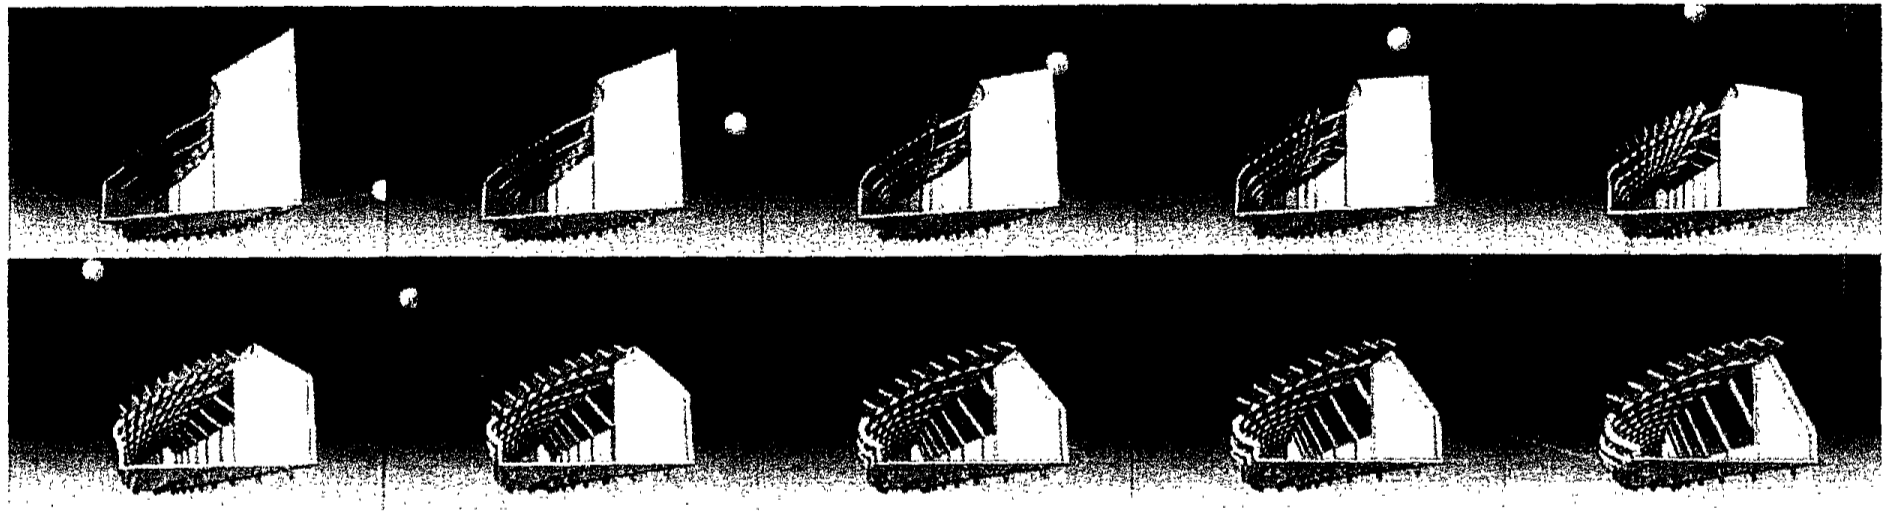
\includegraphics[width=\textwidth]{./Images/7-FinalPavilion}
\caption[Adaptable Pavilion Design Results]{The Adaptable Pavilion \cite{zulas04}}
\label{fig:FinalPav}
\end{figure}

\newpage
\subsubsection{The Kendall Pavilion}

The following is a comprehensive exercise to create an adaptable responsive system, with an approach combining the following concepts and control mechanisms:

\begin{enumerate}
\item Programming objects using Shape Grammar.
\item Conventional programming through coding or scripting.
\item Modelling a real-world situation corresponding to naturally occurring phenomena.
\end{enumerate}

The task is to design an architectural envelope capable of performing responsive geometrical reconfiguration based on the idea of adaption in relation to a geographical location, urban context, and to specific design intentions, responding to the designer's direct manipulation.

\paragraph{The Urban Context Description}

The space designated to locate the pavilion is surrounded by and high and medium sized structures.

\begin{figure}[htbp]
\centering
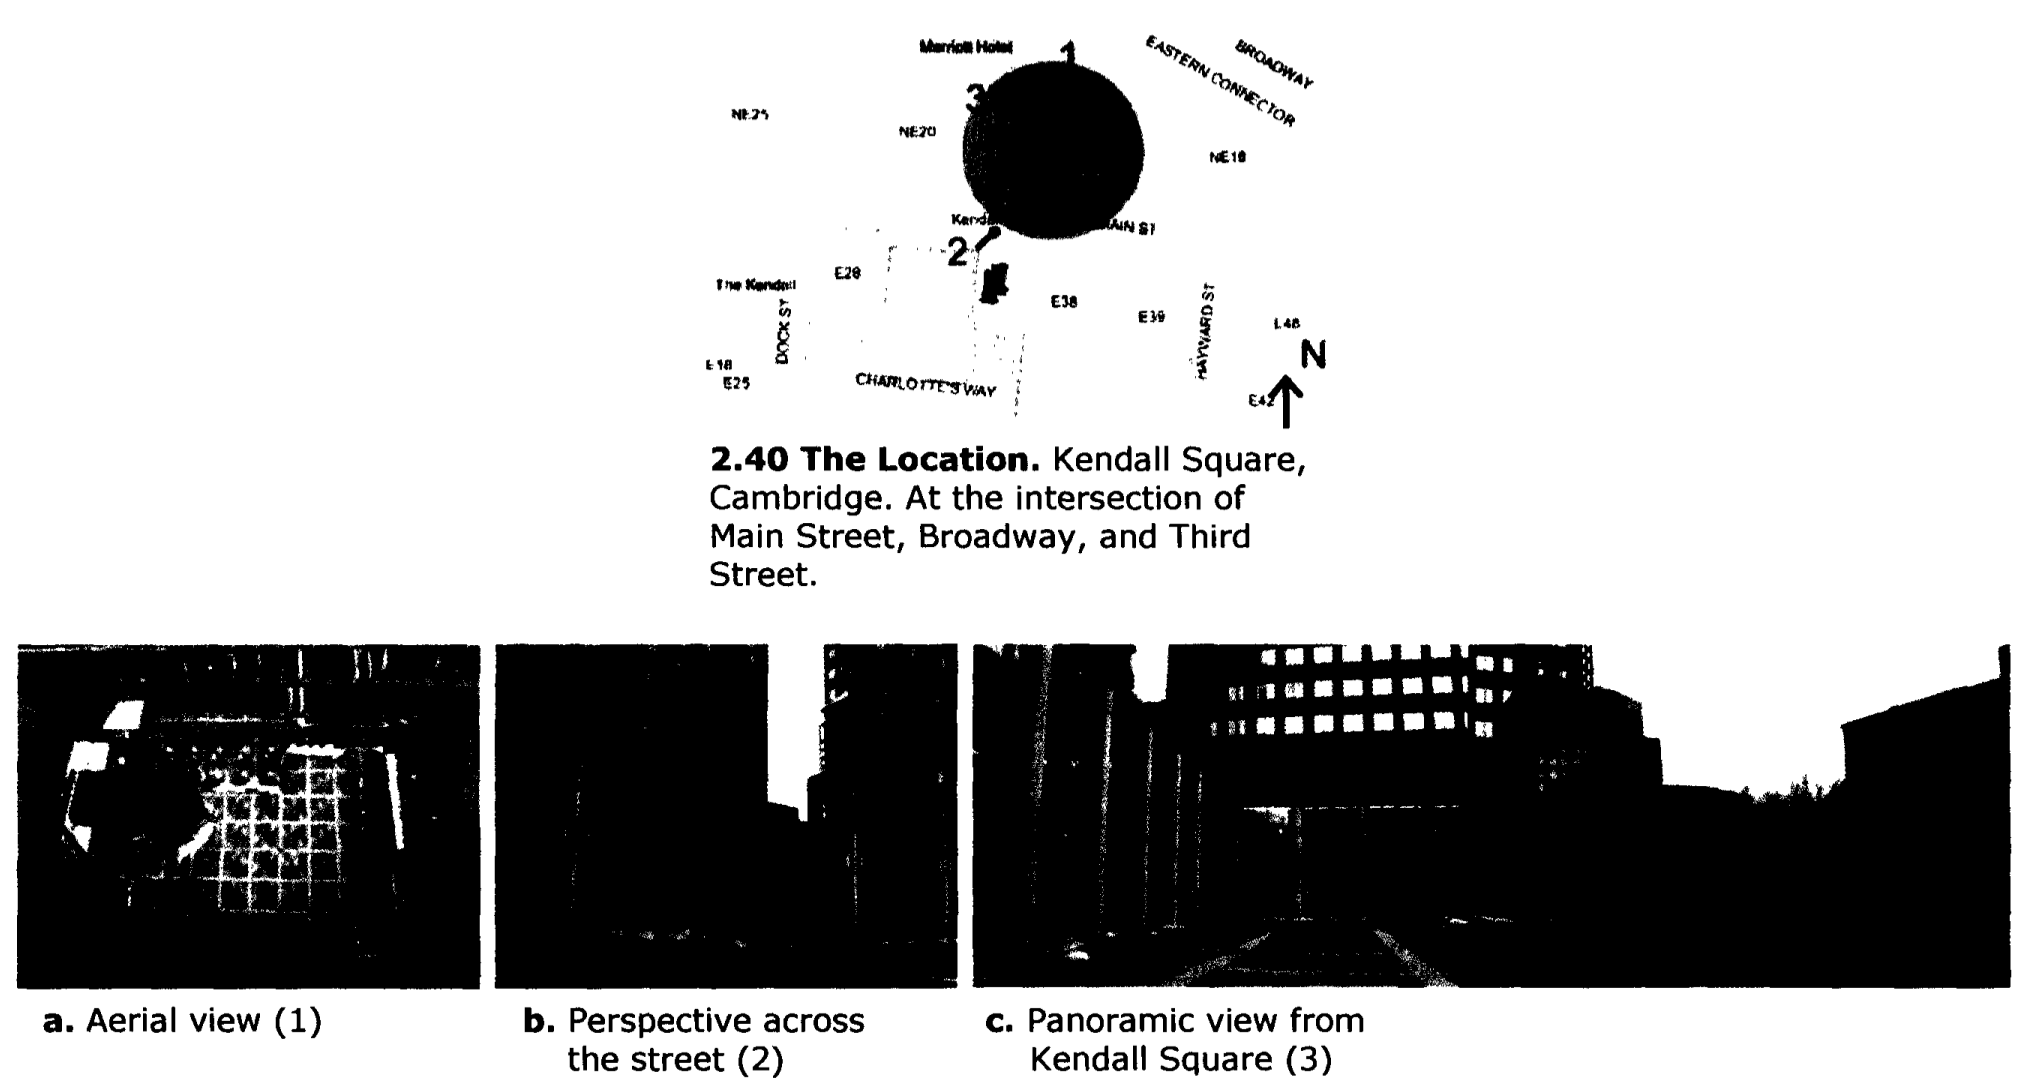
\includegraphics[width=\textwidth]{./Images/8-LocUrban}
\caption[Kendall Pavilion Location and Urban Context]{Location and Urban Context \cite{zulas04}}
\label{fig:KedLoc}
\end{figure}

\paragraph{The Design Intentions} 
\vspace{-0.3cm}
\begin{enumerate}
\item Generate an architectural skin.
\item Embed ``sensory intelligence'' into the building, providing it with object recognition capabilities (surrounding buildings and pedestrian paths) and sun location responsiveness.
\item Embed ``structural intelligence'' into the building skin system, recognising and fixing potential structural instabilities, due to the fact that the building will suffer geometrical reconfiguration while responding to stimulus.
\end{enumerate}
\vspace{-0.4cm}
(See fig. \ref{fig:KenPavDesInt})

\begin{figure}[htbp]
\centering
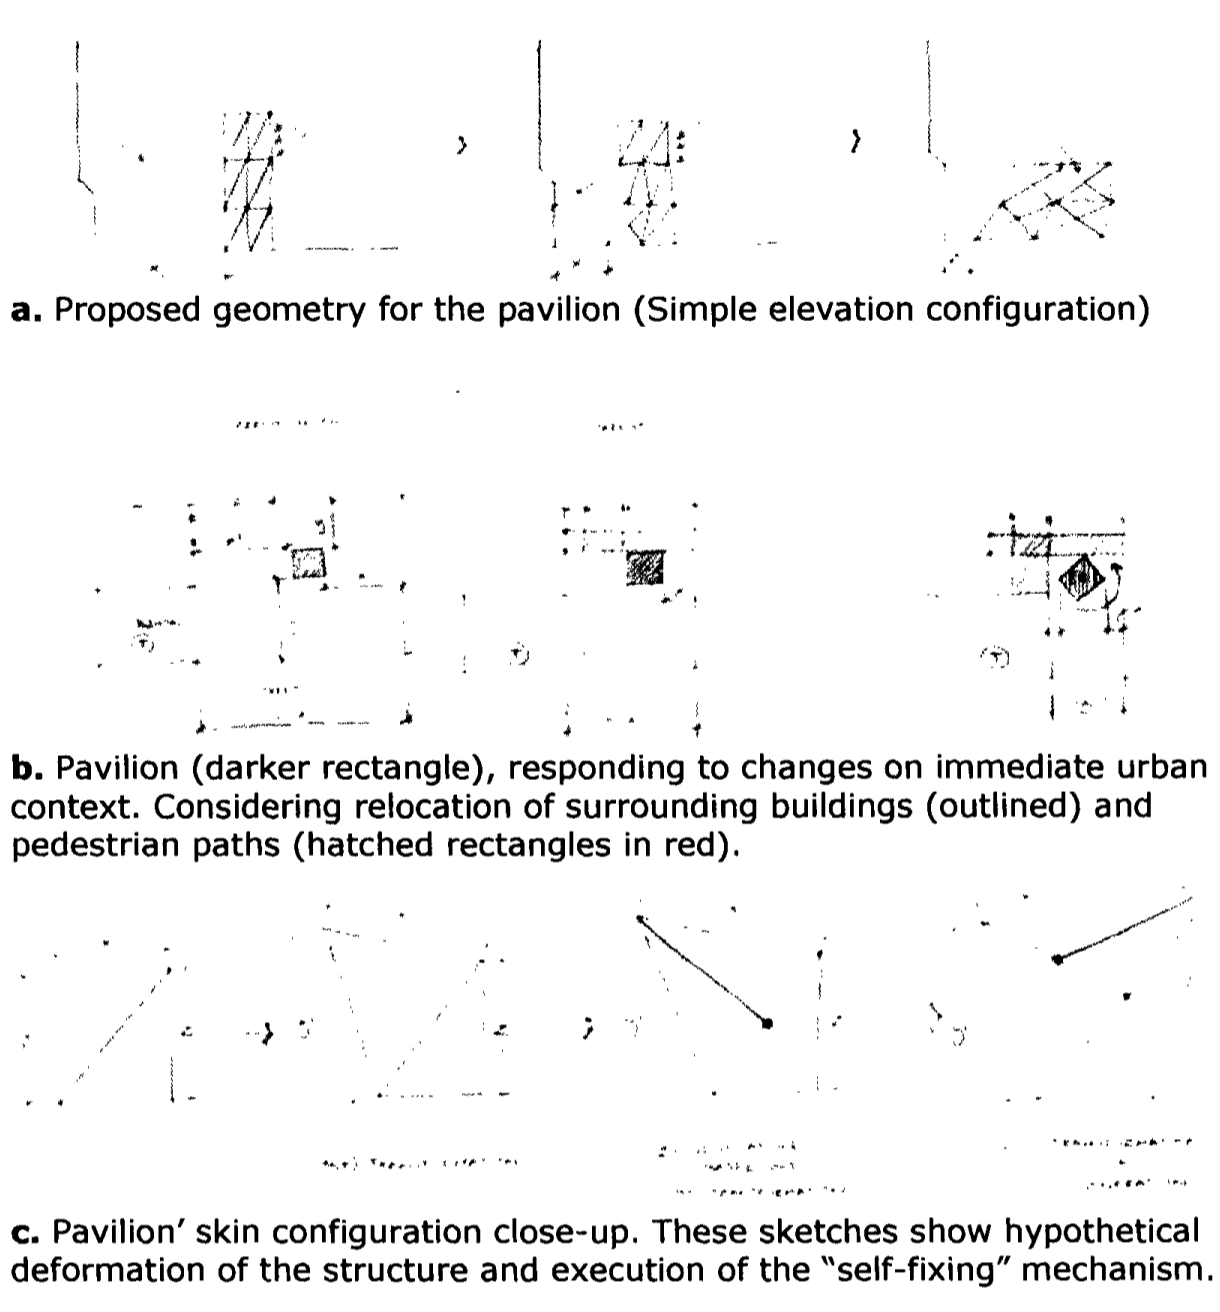
\includegraphics[width=0.7\textwidth]{./Images/9-DesInt}
\caption[Kendall Pavilion Design Intentions]{Kendall Pavilion Design Intentions \cite{zulas04}}
\label{fig:KenPavDesInt}
\end{figure}

\paragraph{The Mapping Process}

As the building will be corresponding to different stimulus, the cause and effect sequence had to be programmed, and four elements were selected as inputs:
\vspace{-0.3cm}
\begin{itemize}[nolistsep]
\item Program
\item Context
\item Environment
\item Designer Input
\end{itemize}
\vspace{-0.4cm}
(See fig. \ref{fig:MapProcs})

\begin{figure}[htbp]
\centering
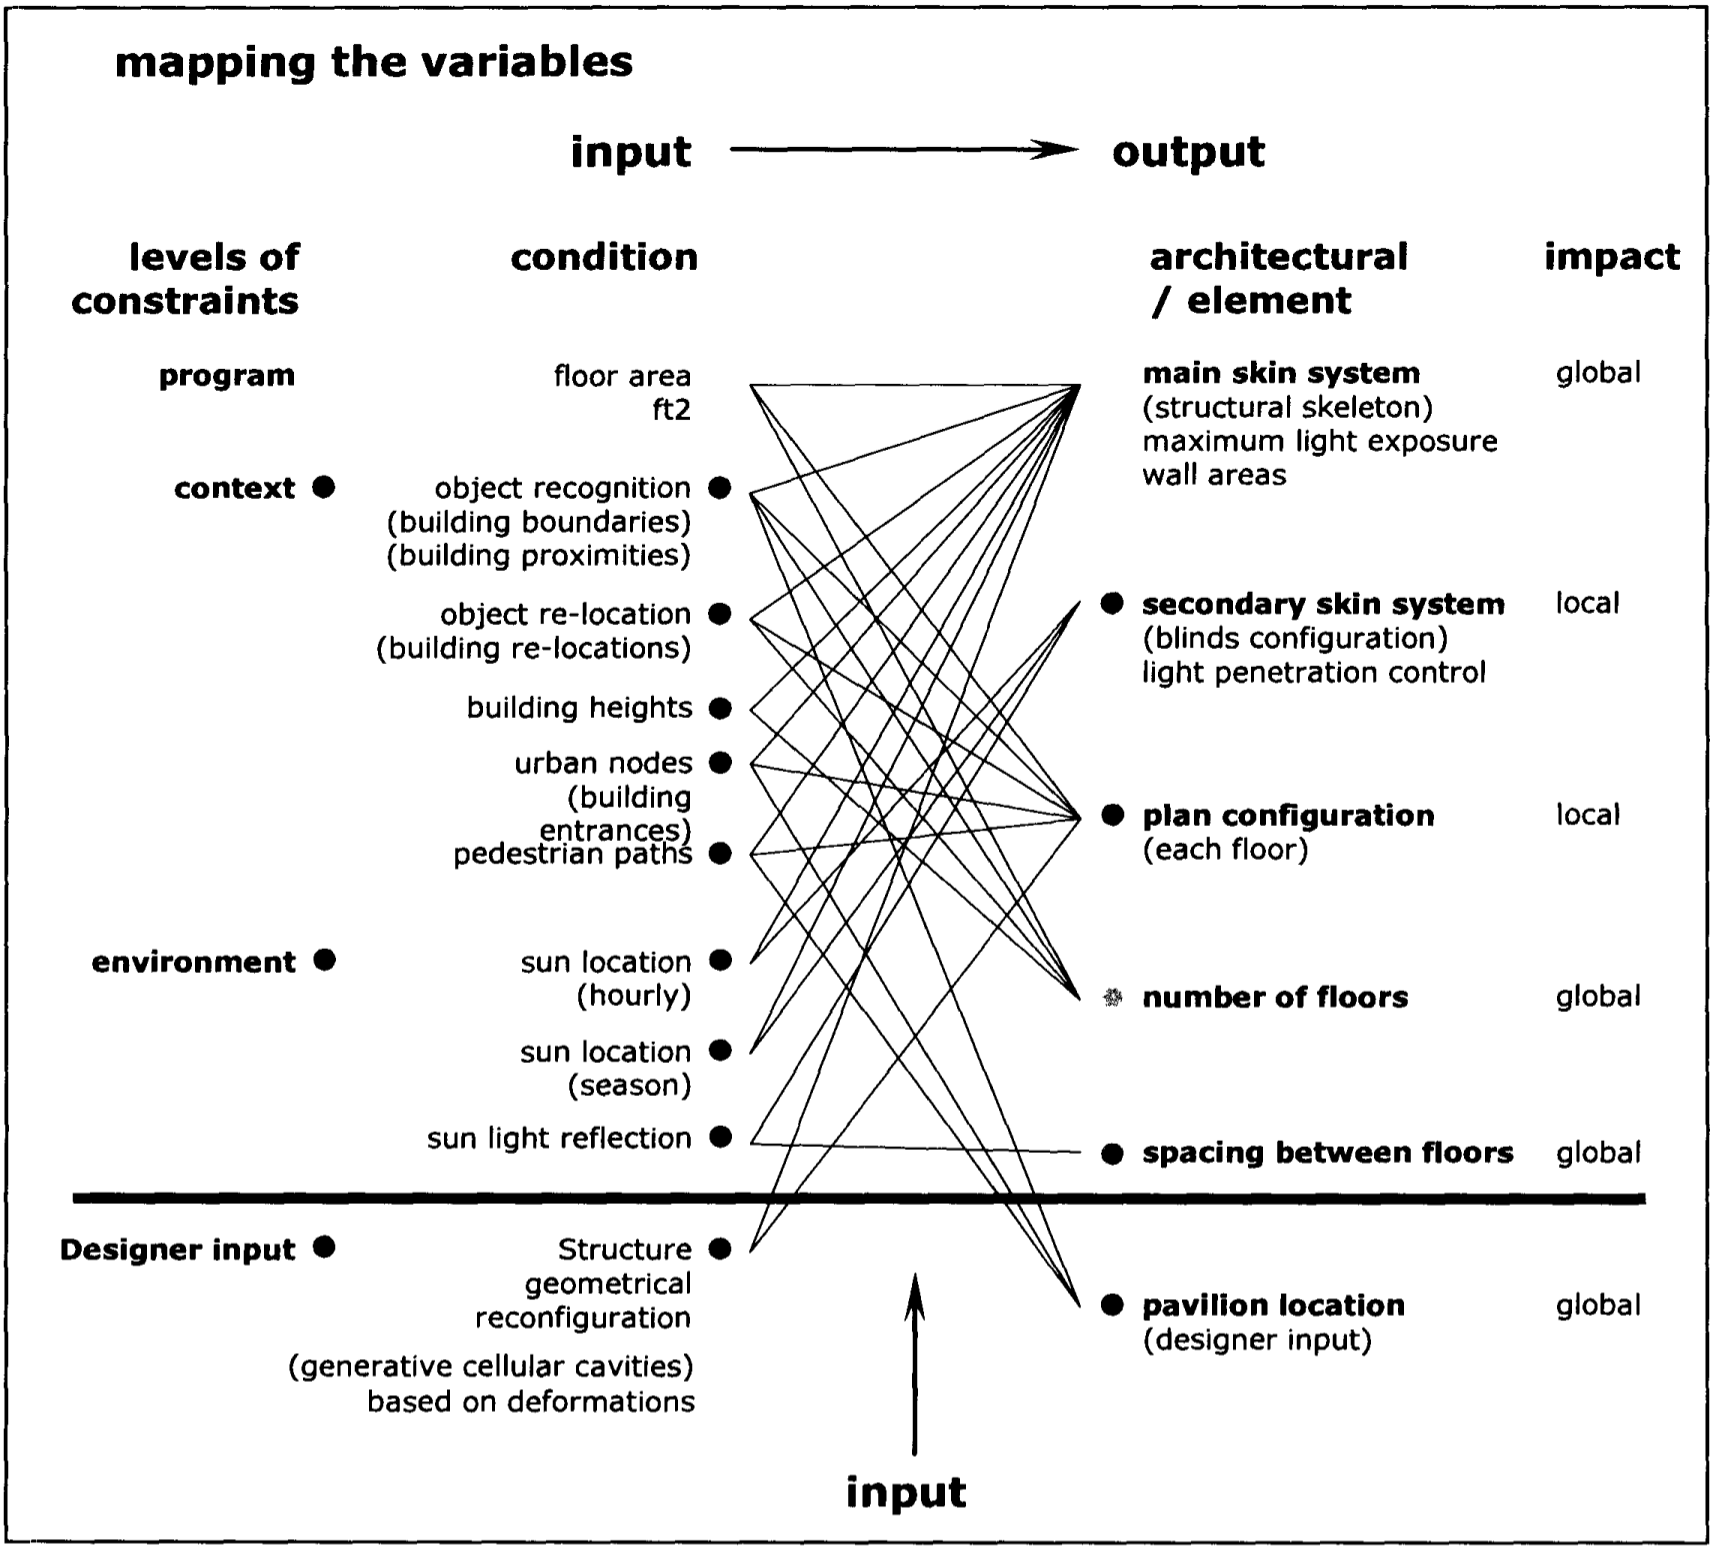
\includegraphics[width=\textwidth]{./Images/10-MapProcs}
\caption[Input/Output Mapping Process]{Input/Output Mapping Process \cite{zulas04}}
\label{fig:MapProcs}
\end{figure}

The author then continued to map the interrelationships of the architectural elements. This was due to the fact that each of the architectural elements would continue to affect each other in a continuous loop indirectly (fig. \ref{fig:ArchElmLoop}).

\begin{figure}[htbp]
\centering
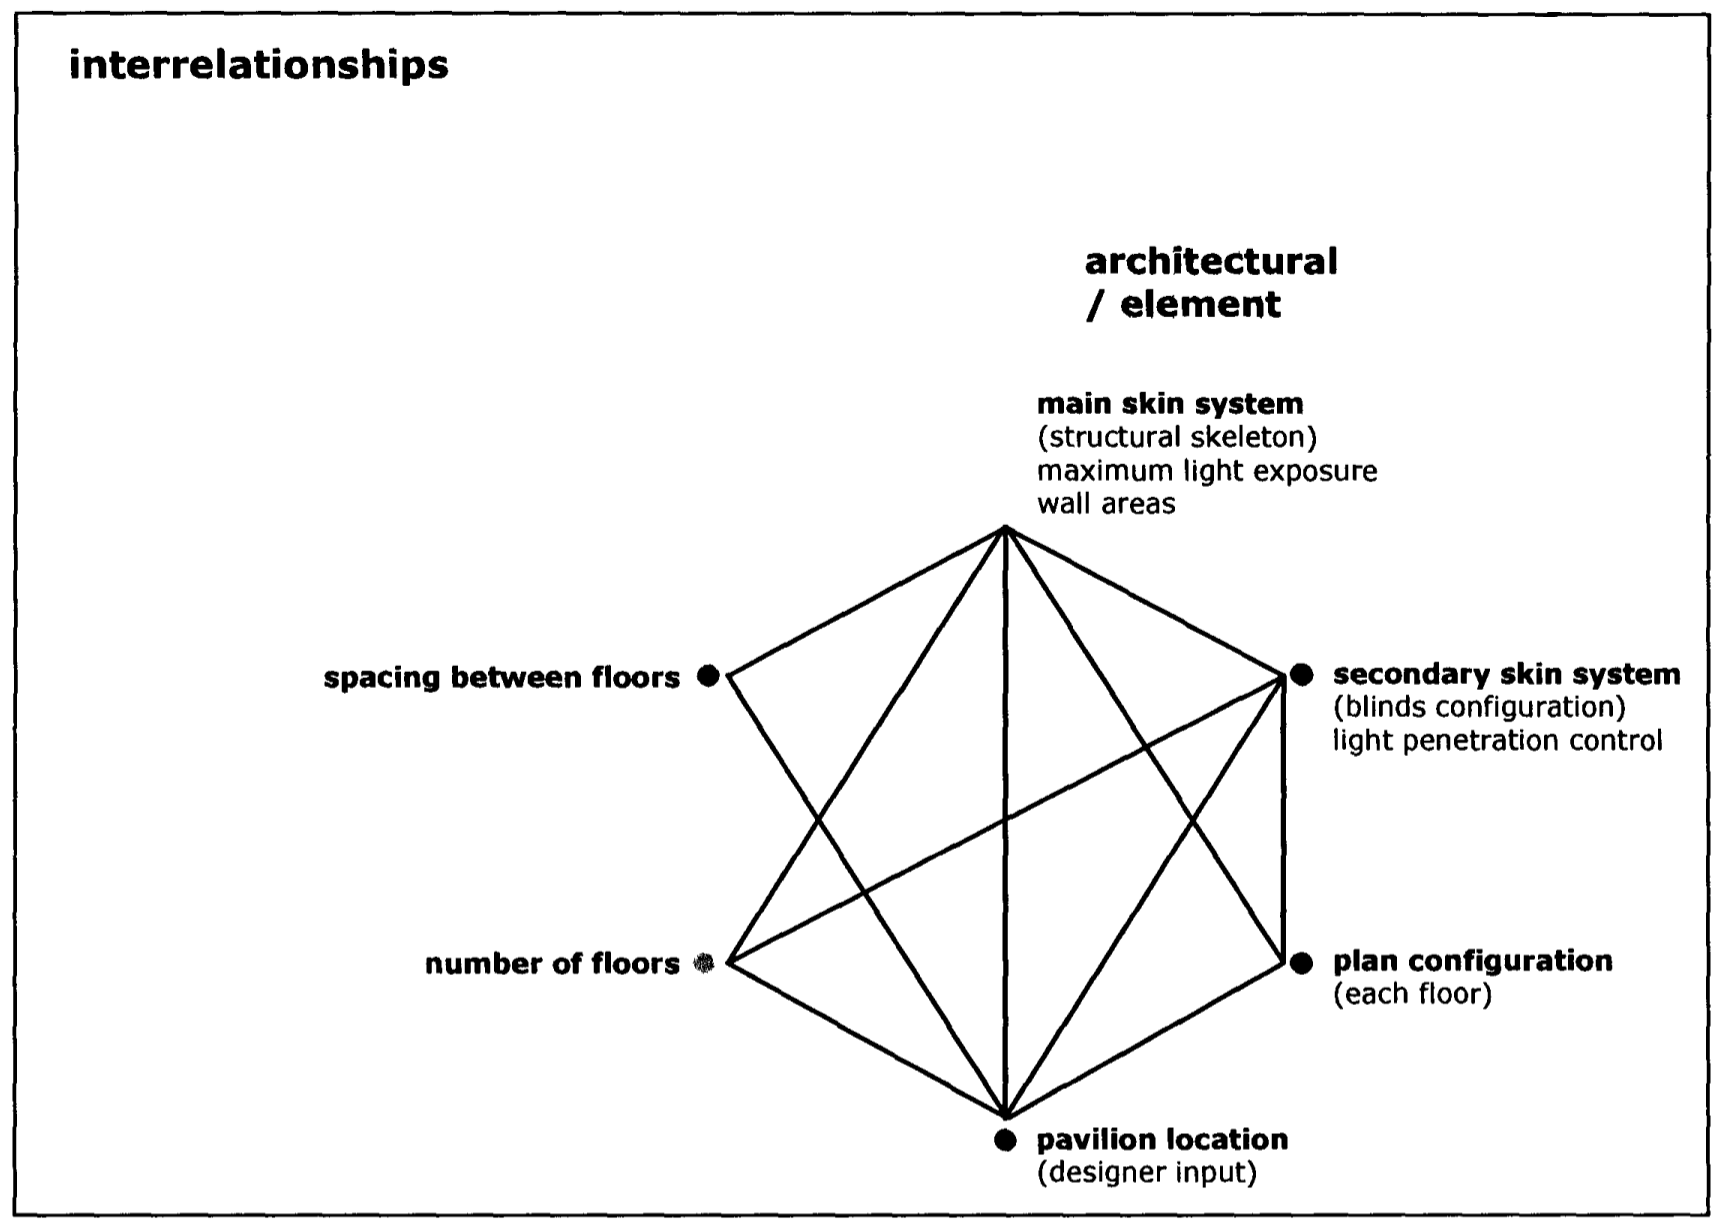
\includegraphics[width=\textwidth]{./Images/11-ArchElmLoop}
\caption[Architectural Elements Interrelationships]{Architectural Elements Interrelationships \cite{zulas04}}
\label{fig:ArchElmLoop}
\end{figure}

\paragraph{Control Mechanisms.}

Having defined the variables and mapping their interrelationships; the next step was to model the data and program the control algorithms. This process was inline with all the design intents mentioned earlier, namely: 
\begin{inparaenum}
\item ``embedding ``sensory intelligence'' in order to achieve object recognition. To be achieved through contextual based conditional,
\item embedding ``smart flexibility'' allowing the user to intervene directly and freely with virtual objects throughout the design process. Implementing the concept of stretchable surfaces (to be further explained),
\item embedding ``structural intelligence in order to achieve specific self-fixing capabilities. Introducing the concept of emergence, to be implemented locally through a rule based approach (to be further explained).''
\end{inparaenum} \cite{zulas04}

The computational approaches that were used to tackle the three concepts stated above were: 

\begin{enumerate}[nolistsep]
\item Parametric representation of context
\item Parametric delimited action: Semi-automated human intervention
\item Generative emergence rules
\end{enumerate}

\subparagraph{Parametric representation of the context.} In order for the system to be ``adaptive'' and ``responsive'', the context should be variable, and therefore parameterised. In the earlier work by the author (refer to section \ref{sec:AdptPav}) the stimulus to which the building had responded was the sun and its movement. Here however, the whole context of buildings, roads and the rest of the stimuli mentioned earlier will affect the buildings response (see fig. \ref{fig:ParametricKendallSq}).

\begin{figure}[htbp]
\centering
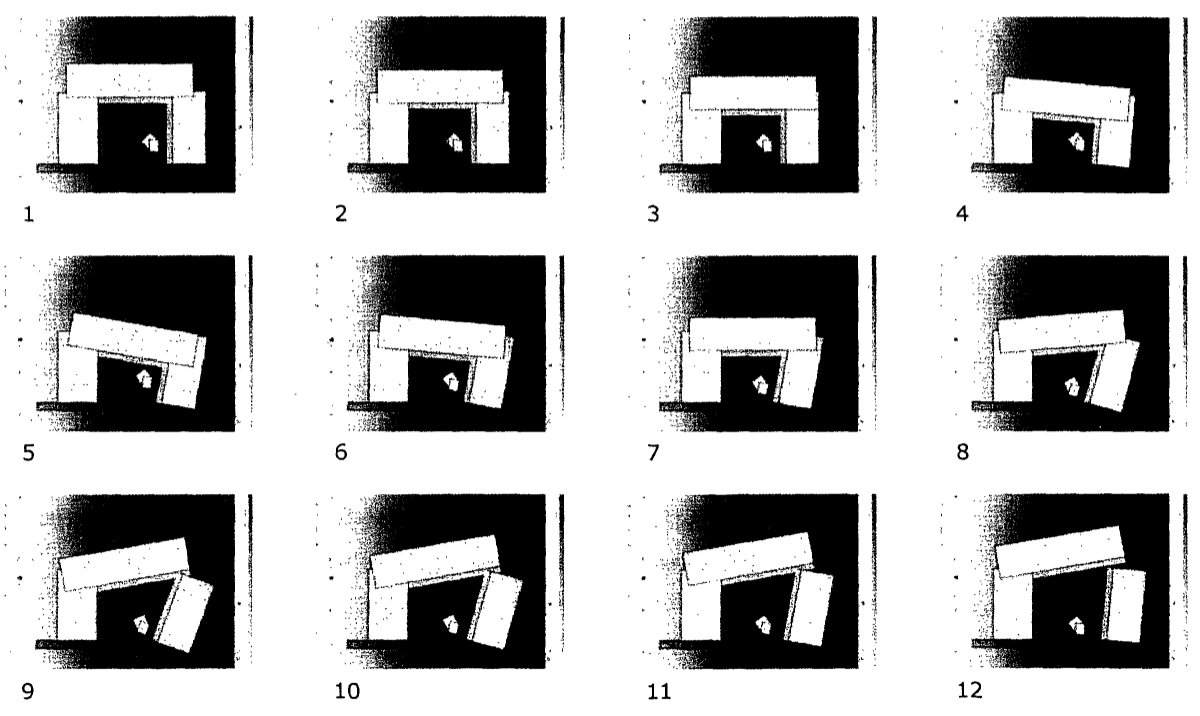
\includegraphics[width=\textwidth]{./Images/12-ParametricContext}
\caption[Parametric Context]{A plan view of the Kendall Square area being manipulated to generate different context through parametric controls \cite {zulas04}}
\label{fig:ParametricKendallSq}
\end{figure}

\begin{figure}[htbp]
\centering
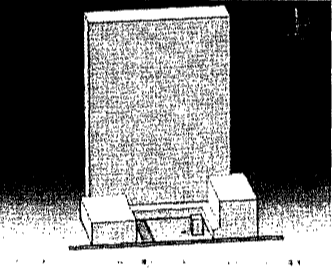
\includegraphics[width=0.4\textwidth]{./Images/13-KendallIsometric}
\caption[Kendall Square Isometric]{An isometric of the Kendall Square \cite{zulas04}}
\label{fig:KendallIsom}
\end{figure}

The parameterisation of the context was achieved by applying a stretchable two-dimensional grid, or net, of lines on the surrounding buildings and pedestrian paths. The method is referred to by the author as manipulation through ``stretchable surfaces''.

\subparagraph{Delimited Action: Semi-automated Human Intervention.}
The ``stretchable surfaces'' concept was further incorporated into the system by making adaption of the pavilion respond to any changes in the grid, which would act as a guide to the programmed adaption algorithm, while allowing direct adjustments to the grid by the designer; hence, a ``semi-automated'' human intervention.

\subparagraph{Generative Emergence Rules.} As mentioned earlier in this chapter; draughting and modelling programs usually provide generative modelling through scripting (end-user programming languages). In this case the author \cite{zulas04} utilised the scripting capabilities of CATIA (parametric modelling application). The emergence rule acts as a form of ``structural intelligence'' (a concept described earlier) where the rule identifies the length of two sides of the basic composition of the pavilion's main structure; which if they are exceeded the system will automatically add an emergent structural element to preserve structural integrity. The script used is shown in fig. \ref{fig:EmergRuleScr}.

\begin{figure}[htbp]
\centering
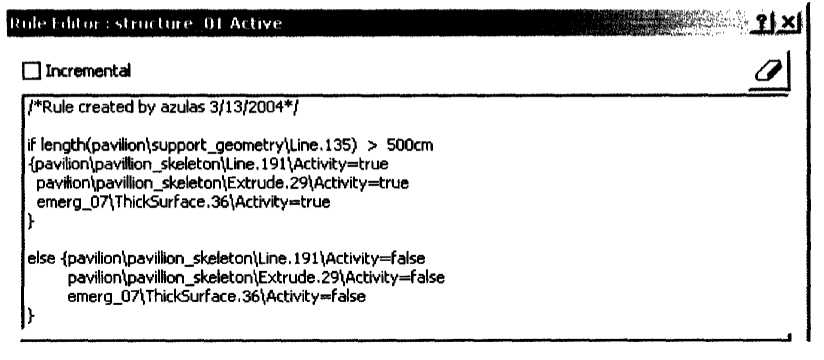
\includegraphics[width=0.7\textwidth]{./Images/14-EmergRuleScr}
\caption[Emergence Rule Script]{A screen capture of the script used in CATIA to apply the emergence rule \cite{zulas04}}
\label{fig:EmergRuleScr}
\end{figure}

\clearpage
\subsection{The ``Generative System'' Search, Optimisation and Simulation System}

The following experiment is part of the research done by Luisa Gama Caldas \cite{caldas01}, in the efforts to create what was called a ``Generative System'', consisting of two main components: \begin{inparaenum} \item a search and optimisation module, and \item a simulation module \end{inparaenum}.

The author chose Genetic Algorithm---abbreviated: GA---(see sec. \ref{subsec:GA}) for the search and optimisation module, which feeds the initial input along with building parameters into the simulation program DOE (see sec. \ref{par:DOE}) which evaluates the results and returns its fitness function value (in this case the annual energy consumption of a building) into GA, which in turn searches the solution space until it reaches the last population\footnote{For explanation of GA terminology; refer to section \ref{subsec:GA}}, the results are then inspected using a visualisation program (see fig \ref{fig:GSfitFun}).

\begin{figure}[htbp]
\centering
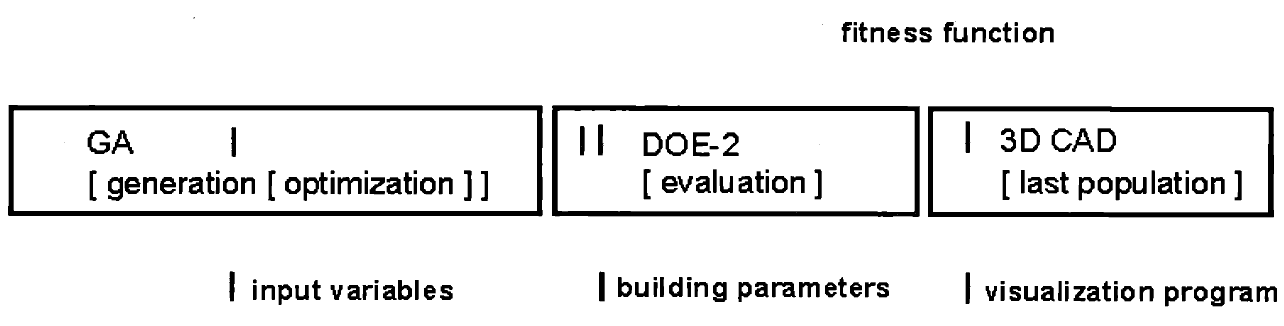
\includegraphics[width=\textwidth]{./Images/15-FitnessFunction}
\caption[GS Information Flow]{The flow of information across the Generative System components \cite{caldas01}}
\label{fig:GSfitFun}
\end{figure}

\paragraph{The Simulation Module: DOE2.1E -- Capabilities and Limitations.} DOE2.1E was chosen as the simulation module for its capability to perform thermal calculations, namely: thermal loads, HVAC loads, extensive material modelling capabilities, library of HVAC systems, and also for its accuracy and reasonable computation times. However, DOE2.1E is incapable of other thermal design related calculations such as Computational Fluid Dynamics [CFD] which simulates air movement and its thermal effects. Another missing feature in DOE is the capability to calculate and predict thermal comfort. 

The author performing the experiment had recommended Energy Plus (see sec. \ref{par:EnergyPlus}) as a replacement of DOE for the above mentioned reasons---in addition to others--- which was not used as it was not available at the time when the experiment was performed.

In the context of this thesis however, the aspects of air movement and ventilation have been disregarded for the sake of simplicity of illustration of generative systems and thermal design integration, and therefore, the simulation of static thermal properties of buildings will suffice in this example.

\paragraph{The Search Module: Genetic Algorithm -- description, advantages and shortfalls} Genetic Algorithm had been chosen by the author as the search and optimisation module due to that GA provides a final `population' of solutions, not a single solution. As stated by the author: ``\emph{A system that would provide a single `optimised' solution might have poor acceptance among architects, who might prefer to have a range of choices between different solutions, all having a high standard of performance according the objective functions included in the search, and from where the architect could exert further choice, according to other criteria like personal preference, initial design intention \ldots etc}.'' (refer to sec. \ref{subsec:OptimComp} for comparison between GA and other search and optimisation methods by Caldas \cite{caldas01}).

Another advantage of GA is the coding of variables in the search process, which applies to binary GA's using binary code---1's and 0's---in its chromosomes. The chromosomes can be encoded into any kind of variable, numerical or non-numerical; for example, part of the chromosome can be encoded as a material name, or a dimension, or into any other kind of numerical or non-numerical variable.

This section will expand on the discussion of GA basic operators: reproduction, crossover and mutation (see sec. \ref{subsec:GA}). The most common implementation of reproduction is called \emph{The Biased Roulette Wheel}, where each current string in the population has a roulette wheel slot sized in proportion to its fitness; that means that the probability of a given individual being selected for reproduction is proportional to its fitness:

\begin{equation}
P(x)=f(x)/ \sum\limits_{j=1}^n f(j) 
\label{eqn:BiasedRoulette}
\end{equation}
\small Where $n=$ number of individuals in the generation
\normalsize

This method of selection and reproduction is usually combined with other methods to determine which individuals will pass to the next generation, such as \emph{Deterministic Tournament Selection}, where two randomly selected strings are set against each other, and only the one with the highest fitness moves to the next generation.

Other notable reproduction methods include: \emph{Multi-Parent Reproduction, Parallel Steady-State Reproduction,} and \emph{Gradient-like Reproduction}.

After reproduction, comes Crossover, which is responsible for diversification during the search process, and is the most prominent operator in GA. During crossover, parts of randomly selected chromosomes are swapped to create a new individual (refer to table \ref{CRSOVR}). Only an elite solution\footnote{A solution with the highest fitness value of the current generation} is passed to the next generation without crossover. The purpose of crossover is to create new points in the solution space through interchange of information between different solutions, which is vital to the success of the search as the elimination of solutions from the limited initial population must be regenerated, and to create diverse generations, expanding the sample space, and increasing the chance of finding the global optimum\footnote{The solution with the highest fitness function value in the entire solution space, as opposed to \emph{Local Optimum} which is the fittest only in the current population}.

Crossover types include \emph{one-point, two-point} and \emph{uniform} crossover; the difference being---respectively---whether the algorithm assigns one crossover point, two crossover points or substitutes the whole string in the following manner:

\begin{equation}
Z=(z_1,\cdots,z_n), z_i=x_i \text{or} z_i=y_i
\label{eqn:UniformCross}
\end{equation}
\small Where $n$ is the chromosome length
\normalsize

Mutation involves changing an \emph{allele}\footnote{One digit of the chromosome string} with a given probability to look for new points in the solution space. Mutation is responsible for introducing information that did not exist in the initial population. Caldas \cite{caldas01} mentions a rule of thumb based on parametric studies, which states that a mutation rate of $m=1/n$, where $n$ is the size of the chromosome; is almost optimal.

\subsubsection{Previous Attempts of Optimisation through Building Energy Simulation Programs}

The researcher continues to illustrate previous work done prior to her research, with the attempt to apply energy simulation programs to create optimum solutions. One of the attempts include the use of DOE-2.1E to optimise design parameters of a window, which relies on indices and weight factors creating a single figure by which the design is evaluated. The indices were: \begin{inparaenum} \item fuel usage, \item electricity usage, \item peak electricity demand, \item thermal comfort, and \item visual comfort \end{inparaenum}. The idea of combining the five indices into one figure however was deemed dubious by the researcher. Thermal comfort was calculated as a correlation between magnitude of solar radiation and the percentage of dissatisfied people. Visual comfort was done through calculation of the glare index.

\subsubsection{Building the Generative System}

The method used by the researcher was to link Genetic Algorithm and DOE-2.1E, where GA would call DOE-2.1E whenever calculation of the fitness of an individual is needed; the fitness function being the \textbf{annual energy consumption}. DOE-2.1E would then run a thermal and lighting simulation of the building under study with the parameters determined by the individual chromosome of that solution. 

A method of data exchange between GA and DOE was developed; different procedures were used for numerical variables, such as dimensions or coordinated, in addition to non-numerical variables.

Non-numerical variables such as material names encoding design was handled with special attention to the relation between the material properties and the binary code. For example; if the number of material selections was 16, 4 alleles would be used ($2^4=16$), so that a material designation would be something like 0101. Each of the 4 alleles would have a specific designation; for example, the first digit would designate if it's an insulation material, the second would designate high or low conductivity \ldots\hspace{0cm}etc.

Another problem was how to incorporate architectural language into the algorithm. Although DOE uses what is called \emph{The Building Description Language} (BDL) as an input format to describe building geometry, it does not allow incorporation of information describing the relations between the different variables under study. Therefore, the constraints of architecural design had to be encoded inside GA code.

\subsubsection{Input and Output Formats}

Since GA had no designed user interface, the input process was text-based. Input consisted of two main steps; namely, creating a DOE-2.1E input file describing the building---including geometry, orientation, space layout, construction material \ldots\hspace{0cm}etc.---and also providing informatino on electrical and mechanical systems to be used in schedules. This was created with nill values assigned to the different variables under study, which would be created by the algorithm. Each of the variables is represented by a numerical value.

The second step would be to adapt the GA to the problem under study, as well as the input files it reads during execution. A function in the source code would call DOE, and pass the right number of arguements to it in correct order. Some relations between different variables are specified. 

Finally, the input files GA reads are modified to identify the variables to be considered in the search, the upper and lower boundaries of each variable, the number of intermediate steps between those limits and the number of binary bits required to code each variable. Also, a file would be included that defines the population size in GA, and the number of generations, in addition to other control mechanisms of the search process.

The output is then passed on to either an AutoLisp routine which draws an AutoCAD file from the results, or through a program called DrawBDL which generates a 3D model from DOE output files.

\subsubsection{Testing the Generative System}

For the experiment, a simple schematic building consisting of a core area with surrounding rooms facing each of the four main cardinal orientations\footnote{North, South, East and West}; each room had a single window looking on the opposite side of the core (see fig. \ref{fig:SchmBuild}).

\begin{figure}[htbp]
\centering
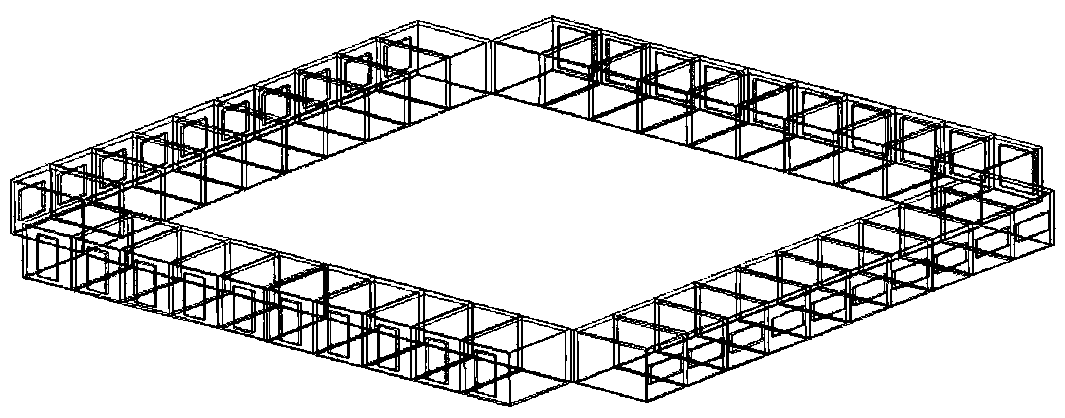
\includegraphics[width=\textwidth]{./Images/16-SchematicBuilding}
\caption[GS Schematic Building]{GS Schematic Building \cite{caldas01}}
\label{fig:SchmBuild}
\end{figure}

\paragraph{Simulation Method}\mbox{}\\

A framework is designed for the genetic algorithm to allow for enoding and manipulation of variables which suits the problem. To be able to utilise GA; it was necessary to provide the following:
\begin{enumerate}
\item A binary string of bits
\item An objective function definition, which would pass the data to DOE
\item Mechanisms for selection, crossover and mutation
\item Choosing initial population size, and
\item Maximum number of generations.
\end{enumerate}

\subparagraph{Representation of feasible solutions.} The building has
